\documentclass[11pt, a4paper,titlepage]{article}
\usepackage[a4paper,top=1.5cm,bottom=1.5cm,left=2cm,right=2cm]{geometry}
%% Declaro simbolo
\usepackage[T1]{fontenc}
\newcommand{\rmfont}[1]{{\fontfamily{ptm}\selectfont%
#1}}
\newcommand{\rmfontbf}[1]{{\fontfamily{ptm}\selectfont%
\textbf{#1}}}
\newcommand{\rmfontsc}[1]{{\fontfamily{ptm}\selectfont%
\textsc{#1}}}

%%----------------------------------------------------

	\usepackage[spanish]{babel}
	\selectlanguage{spanish}
   
	\usepackage[utf8]{inputenc} % Aca va el setup para el codigo.
    \usepackage{graphicx}
    \usepackage{upquote}% esto tampoco creo
    \usepackage{amsmath,array,siunitx}
    \newcommand{\vvert}[1]{\left\Vert #1\right\Vert}
    \usepackage{listings}
	\usepackage{mdframed}
	\usepackage{xcolor} 
    \usepackage[utopia]{mathdesign}
    \newcommand{\Matlab}{\rmfont{\sc Matlab}}
    \newcommand{\Adina}{{\sc ADINA}}
    \newcommand{\refp}[1]{(\ref{#1})}
    \newcommand{\unspace}{\!\!\!\!\!\!\!\!\!\!\!\!\!\!\!\!\!\!\!\!}
    \newcommand{\ms}{\ \ \ } %Matrix Spacing
    \newcommand{\di}{\textrm{d}}
    \newcommand{\jac}{\rmfontbf{J}}
    \newcommand{\Djac}{|\;\jac\;|}
    \newcommand{\dNi}{\di N_i}
    \newcommand{\sigmab}{\boldsymbol{\sigma}}
    \newcommand{\varepsilonb}{\boldsymbol{\varepsilon}}
    \newcommand{\Phib}{\boldsymbol{\Phi}}
    \newcommand{\COmega}{\boldsymbol{\{ } \Omega \boldsymbol{\} }}
    \newcommand{\CPhi}{\boldsymbol{\{ } \Phi \boldsymbol{\} }}
    \newcommand{\Mme}[1]{\boldsymbol{[}\mathbf{#1} \boldsymbol{]}}
    \newcommand{\Rme}[1]{\boldsymbol{\lfloor}\mathbf{#1} \boldsymbol{\rfloor}}
    \newcommand{\Cme}[1]{\boldsymbol{\{ }\mathbf{#1} \boldsymbol{\}} }
    \newcommand{\MB}{\Mme{B}}
    \newcommand{\MN}{\Mme{N}}
    \newcommand{\ME}{\Mme{E}}
    \newcommand{\Mk}{\Mme{k}}
    \newcommand{\MA}{\Mme{A}}
    \newcommand{\radial}{r}
    \newcommand{\eff}{f}
    \newcommand{\modal}{{_{\Phib}}}
    \newcommand{\dampfact}{\varsigma}
    
\newmdtheoremenv[% ACA PODES MODIFICAR LAS PROPIEDADES DEL CODIGO {code}
font=\fontsize{12pt}{16pt},
linecolor=black,
leftmargin=-.9cm,%
rightmargin=-.9cm,
backgroundcolor=gray!5,%
innertopmargin=8pt,%
ntheorem]{code}{Codigo}[section]
%-----------------------------------------------------------
\begin{document}  %Aqui empieza el documento
\begin{titlepage} %Esta es la caratula
\centering
{\scshape\Huge Elementos Finitos Cheatsheet \par}
\vspace{1cm}

\vspace{2cm}
{\scshape\Large\textbf{Autores} \par}
\medskip %medskip,smallskip,vspace son todos comandos para dejar espacio en blanco entre cosas
 \textsc{55423}

\end{titlepage} %Termina la caratula


%\bgroup
\section{Parcial 1}

\begin{code}[Inicializar]
\begin{verbatim}

nod=[0 0;0 L;0 2*L;-L L;-L 2*L;-1.5*L 0;-1.5*L L;-1.5*L 2*L];
N=length(nod);
R=zeros(length(nod)*3,1); %hinges! 
elenod=[8 5;5 3;7 4;4 2;7 6;5 4;5 2;4 1;3 2;2 1];
CB=false(N*3,1); %add hinges
nodo=@(n) [n*3-2 n*3-1 n*3]; %gr8 func
CB(nodo(8))=~~[1 0 1]';
\end{verbatim}
\end{code}

\subsection{Variable Generation}
%\includegraphics[width=\textwidth]{1zunch.pdf}

\begin{code}
\begin{verbatim}

function [nodeDofs,elenod,nudos,Le,phide,Ndof] = ...
gennodedofs(nod,elenod,eletype)
%GENNODEDOFS genera matriz nodeDofs
[Ne,~]=size(elenod);
[N,~]=size(nod);
hinges=length(eletype(eletype==4 | eletype==44 | eletype==3 | eletype==33));
Le=zeros(Ne,1);
phide=zeros(Ne,1);
Ndof=N*3+hinges;
%HINGES (ROTULAS)
hingedlist=zeros(1,hinges);
j=0;
Nt=N+hinges;
nodeDofs=zeros(Nt,3);
nudos=zeros(Nt,1);
for i=1:N
    nodeDofs(i,:)=[i*3-2 i*3-1 i*3];
end
%Termino de llenar nodeDofs y lleno nudos
for i = 1:Ne
    nodestart=elenod(i,1);
    nodeend=elenod(i,2);
    lx=nod(nodeend,1)-nod(nodestart,1);
    ly=nod(nodeend,2)-nod(nodestart,2);
    Le(i)=sqrt(lx^2+ly^2);
    phide(i)=atan2d(ly,lx);%angulo en degrees
    switch eletype(i)
        case {2,22}
            nudos(nodestart)=nudos(nodestart)+1;
            nudos(nodeend)=nudos(nodeend)+1;
        case {3,33}
            j=j+1;
            nudos(nodeend)=nudos(nodeend)+1;
            hingedlist(j)=i; 
            elenod(i,1)=N+j;
            nodeDofs(N+j,:)=[nodestart*3-2 nodestart*3-1 N*3+j];
        case {4,44}
            j=j+1;
            nudos(nodestart)=nudos(nodestart)+1;
            hingedlist(j)=i; 
            elenod(i,2)=N+j;
            nodeDofs(N+j,:)=[nodeend*3-2 nodeend*3-1 N*3+j];
    end
end
\end{verbatim}% las mierditas de los apostrofes joden mucho.
\end{code}

\subsection{Assembly}
\subsubsection*{Assemble bar}
\begin{code}
\begin{verbatim}

klocal=Kb(Ee(i),Ae(i),Le(i));
if eletype(i)==11
    klocal=klocal/2;
end
T=Tbu(phide(i));
kbarrarotada=T*klocal*T';
index=[nodeDofs(elenod(i,1),[1 2]) nodeDofs(elenod(i,2),[1 2])];
kG(index,index)=kG(index,index)+kbarrarotada;
klocalrotada=kbarrarotada;
index=[nodeDofs(elenod(i,1),[1 2]) nodeDofs(elenod(i,2),[1 2])];
elementos(i,[1 2 3 4 5 6])=...
    [index(1:2) nodeDofs(elenod(i,1),3) index(3:4) nodeDofs(elenod(i,2),3)];
if nudos(elenod(i,1))==0
    CB(index(2)+1)=true;
end
if nudos(elenod(i,2))==0
    CB(index(4)+1)=true;
end
\end{verbatim}
\end{code}
\subsubsection{Assemble beam}
\begin{code}
\begin{verbatim}

klocal=Kv(Ee(i),Ae(i),Ie(i),Le(i));
if eletype(i)>11
    klocal=klocal/2;
end
T=Tvu(phide(i));
klocalrotada=T'*klocal*T;
index=[nodeDofs(elenod(i,1),:) nodeDofs(elenod(i,2),:)];
elementos(i,:)=index;
kG(index,index)=kG(index,index)+klocalrotada;
\end{verbatim}
\end{code}

\subsubsection*{3-D Beam with taxed displacements}

\begin{code}
\begin{verbatim}

nod=[4 4 3; 0 4 3...
enod=[2 1;2 1...
fnod=@(n) [n*6-5 n*6-4 n*6-3 n*6-2 n*6-1 n*6];
[Ne,~]=size(enod);
[N,~]=size(nod);
Le=zeros(Ne,1);
kG=zeros(6*N);
for i=1:Ne
    ns=enod(i,1);
    ne=enod(i,2);
    lx=nod(ne,1)-nod(ns,1);
    ly=nod(ne,2)-nod(ns,2);
    lz=nod(ne,3)-nod(ns,3);
    Le(i)=sqrt(lx^2+ly^2+lz^2);%Long.
    px=[lx ly lz]/Le(i);
    vy=[0 pi 5];
    pz=cross(px,vy)/norm(cross(px,vy));
    py=cross(pz,px);
    C=[px',py',pz'];%Para barras no importa orientacion azimuth (acimutal)
    T=blkdiag(C,C,C,C);
    Ts=[Ts T];
    klocal=Kvuw(Ee(i),Ae(i),0,0,0,0,Le(i));
    krotada=T'*klocal*T;
    kG([fnod(ns) fnod(ne)],[fnod(ns) fnod(ne)])=...
      kG([fnod(ns) fnod(ne)],[fnod(ns) fnod(ne)])+krotada;
end
CB=false(6*N,1);
CB([fnod(2) fnod(3) fnod(4) fnod(5)])=true;
CB(fnod(1))=~~[0 0 0 1 1 1];
Kr=kG(~CB,~CB);
R=zeros(6*N);
R(fnod(1))=[0 -10e3 0 0 0 0];
F=R(~CB);
U=Kr\F;
%Ahora imponemos desplazamiento inicial--------
v1=-1.517731e-04;
Dc=zeros(N*6,1);
Dc(fnod(1))=[0 v1 0 0 0 0];
CB(fnod(1))=~~[0 1 0 1 1 1];
R=zeros(N*6,1); %si hay fuerzas ademas de la desconocida las agregamos
Dx=kG(~CB,~CB)\(R(~CB)-kG(~CB,CB)*Dc(CB));
Rx=kG(CB,CB)*Dc(CB)+kG(CB,~CB)*Dx;
R(CB)=Rx
\end{verbatim}
\end{code}

\begin{code}
\begin{verbatim}

klocal=Kb(Ee(i),Ae(i),Le(i));
if eletype(i)==11
    klocal=klocal/2;
end
T=Tbu(phide(i));
kbarrarotada=T*klocal*T';
index=[nodeDofs(elenod(i,1),[1 2]) nodeDofs(elenod(i,2),[1 2])];
kG(index,index)=kG(index,index)+kbarrarotada;
klocalrotada=kbarrarotada;
index=[nodeDofs(elenod(i,1),[1 2]) nodeDofs(elenod(i,2),[1 2])];
elementos(i,[1 2 3 4 5 6])=...
    [index(1:2) nodeDofs(elenod(i,1),3) index(3:4) nodeDofs(elenod(i,2),3)];
if nudos(elenod(i,1))==0
    CB(index(2)+1)=true;
end
if nudos(elenod(i,2))==0
    CB(index(4)+1)=true;
end
\end{verbatim}
\end{code}
\subsubsection*{Assemble beam}
\begin{code}
\begin{verbatim}

klocal=Kv(Ee(i),Ae(i),Ie(i),Le(i));
if eletype(i)>11
    klocal=klocal/2;
end
T=Tvu(phide(i));
klocalrotada=T'*klocal*T;
index=[nodeDofs(elenod(i,1),:) nodeDofs(elenod(i,2),:)];
elementos(i,:)=index;
kG(index,index)=kG(index,index)+klocalrotada;
\end{verbatim}
\end{code}
\clearpage
\subsubsection*{Matrixes}

\begin{code}
\begin{verbatim}

Tb=[cosd(phi) 0;
    sind(phi) 0;
    0 cosd(phi);
    0 sind(phi)];
    
T=[cosd(phi) sind(phi) 0 0 0 0;
    -sind(phi) cosd(phi) 0 0 0 0;
    0 0 1 0 0 0;
    0 0 0 cosd(phi) sind(phi) 0;
    0 0 0 -sind(phi) cosd(phi) 0;
    0 0 0 0 0 1];
    
    k=E*A/L;
klocal=[k -k;
    -k k];
    
    kv= [A*E/L 0 0 -A*E/L 0 0;
    0 12*E*I/L^3 6*E*I/L^2 0 -12*E*I/L^3 6*E*I/L^2;
    0 6*E*I/L^2 4*E*I/L 0 -6*E*I/L^2 2*E*I/L;
    -A*E/L 0 0 A*E/L 0 0;
    0 -12*E*I/L^3 -6*E*I/L^2 0 12*E*I/L^3 -6*E*I/L^2;
    0 6*E*I/L^2 2*E*I/L 0 -6*E*I/L^2 4*E*I/L];
    
     X=A*E/L;
    G=E/(2+2*nu);
    S=G*K/L;
    Y1=12*E*Iz/L^3;
    Y2=6*E*Iz/L^2;
    Y3=4*E*Iz/L;
    Y4=Y3/2;
    Z1=12*E*Iy/L^3;
    Z2=6*E*Iy/L^2;
    Z3=4*E*Iy/L;
    Z4=Z3/2;
    K=[.5*X 0 0 0 0 0,-X 0 0 0 0 0;
        0 .5*Y1 0 0 0 Y2,0 -Y1 0 0 0 Y2;
        0 0 .5*Z1 0 -Z2 0, 0 0 -Z1 0 -Z2 0;
        0 0 0 .5*S 0 0,0 0 0 -S 0 0;
        0 0 0 0 .5*Z3 0, 0 0 Z2 0 Z4 0;
        0 0 0 0 0 .5*Y3, 0 -Y2 0 0 0 Y4;
        ...
        0 0 0 0 0 0, .5*X 0 0 0 0 0;
        0 0 0 0 0 0, 0 .5*Y1 0 0 0 -Y2;
        0 0 0 0 0 0, 0 0 .5*Z1 0 Z2 0;
        0 0 0 0 0 0, 0 0 0 .5*S 0 0;
        0 0 0 0 0 0, 0 0 0 0 .5*Z3 0;
        0 0 0 0 0 0, 0 0 0 0 0 .5*Y3];
    K=K+K';%simetriza las cosas
\end{verbatim}
\end{code}

\egroup

\section{Parcial 2}
Protip: Necesitas saber que fuerza se tiene que hacer para que se mantenga en posición una arista o punto dado cargas térmicas/fuerza? Apoyalo (fix) y mira las reacciones con la carga termica/fuerza.
\subsection{Expresiones útiles}

\begin{align}
    \sigma_{v}&=\sqrt{\sigma_{x}^2+\sigma_{y}^2+\sigma_{z}^2 - \sigma_x \sigma_y-\sigma_x\sigma_z -\sigma_y \sigma_z +3(\sigma_{xy}^2+\sigma_{xz}^2 +\sigma_{yz}^2)} \\
    \sigma_{v}&=\sqrt{\tfrac{1}{2}\left[  (\sigma_{11}-\sigma_{22})^2+(\sigma_{11}-\sigma_{33})^2+(\sigma_{22}-\sigma_{33})^2\right] +3(\sigma_{12}^2+\sigma_{13}^2 +\sigma_{23}^2)}
\end{align}

\begin{equation}
    \lambda = \frac{E \nu}{(1+\nu)(1-2\nu)} \qquad\quad \mu=G=\frac{E}{2(1+\nu)}
\end{equation}

\begin{equation}
\begin{bmatrix}
    \sigma_{xx} \\
    \sigma_{yy} \\
    \sigma_{xy}
\end{bmatrix}
={\frac{E}{1-\nu^2}} 
\begin{bmatrix}
    1 & \nu & 0 \\
    \nu & 1 &0 \\
    0 & 0 & \frac{1-\nu}{2}
\end{bmatrix}
\cdot
\begin{bmatrix}
    \varepsilon_{xx} \\
    \varepsilon_{yy} \\
    2\varepsilon_{xy}
\end{bmatrix}
\end{equation}

\begin{equation}
\begin{bmatrix}
    \sigma_{11} \\
    \sigma_{22} \\
    \sigma_{12}
\end{bmatrix}
={\frac{E}{(1+\nu)(1-2\nu)}} 
\begin{bmatrix}
    1-\nu & \nu &0 \\
    \nu &1-\nu& 0 \\
    0 & 0 & \frac{1-2\nu}{2}
\end{bmatrix}
\cdot
\begin{bmatrix}
    \varepsilon_{11} \\
    \varepsilon_{22} \\
    2\varepsilon_{12}
\end{bmatrix}
\end{equation}

\begin{equation}
    \sigma_{n}=\frac{\sigma_{xx}+\sigma_{yy}}{2}+\left(\frac{\sigma_{xx}-\sigma_{yy}}{2}\right)\cos 2\theta +\tau_{xy}\sin 2\theta 
\end{equation}

\begin{equation}
    \tau_{n}=-\left(\frac{\sigma_{xx}-\sigma_{yy}}{2}\right)\sin 2\theta +\tau_{xy}\cos 2\theta 
\end{equation}

\begin{equation}
    I=\int^1_{-1} \phi(\xi) \di \xi \approx \phi(\xi_1) W_1+\phi(\xi_2) W_2 \ldots \phi(\xi_n) W_n
\end{equation}
\begin{equation}
    I=\int^1_{-1} \int^1_{-1}\phi(\xi,\eta) \di \xi \di \eta\approx \sum_i \sum_j W_i W_j\phi(\xi,\eta) 
\end{equation}



\begin{tabular}{>{$n=$}l<{ \vspace{10pt}}*{13}{c}}
0 &&&&&&&1&&&&&&\\
1 &&&&&&$x$&&$y$&&&&&\\
2 &&&&&$x^2$&&$xy$&&$y^2$&&&&\\
3 &&&&$x^3$&&$x^2y$&&$xy^2$&&$y^3$&&&\\
4 &&&$x^4$&&$x^3y$&&$x^2y^2$&&$xy^3$&&$y^4$&&\\
5 &&$x^5$&&$x^4y$&&$x^3y^2$&&$x^2y^3$&&$xy^4$&&$y^5$&\\
6 &$x^6$&&$x^5y$&&$x^4y^2$&&$x^3y^3$&&$x^2y^4$&&$xy^5$&&$y^6$
\end{tabular}

\begin{figure}
    \centering
    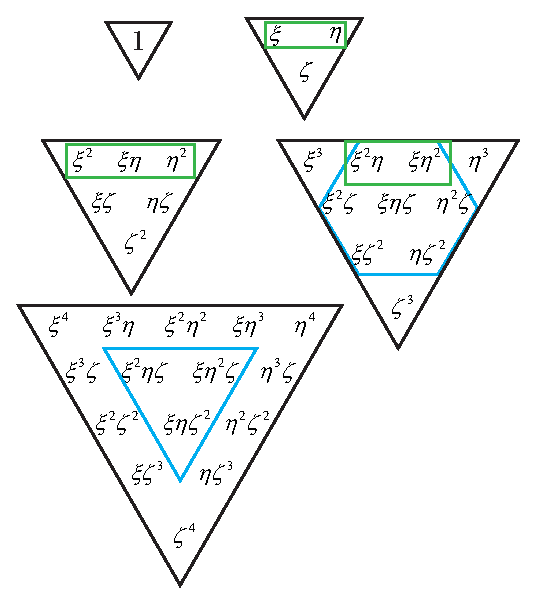
\includegraphics[width=0.5\textwidth]{fig/pascalsTetra.eps}
    \caption{El tetrahedro de Pascal. Los términos de los elementos \textit{serendipidad} están encuadrados.}
    \label{fig:PascalsTetrahedron}
\end{figure}

\subsection{Como obtener cualquier función de forma}
Se define cuantos nodos se va tener por elemento y se los ubica en el espacio $(\xi,\eta)$ que por simplicidad se trataran como $(x,y)$. Con el triangulo de Pascal para polinomios se elige el grado del polinomio y los términos. Luego se resuelve el sistema de ecuaciones $N_i\cdot X= A$ donde $N_i=[N_1\ms N_2 \ms \ldots\ms N_n]$ y $X=[1\ms x\ms y \ms\ldots\ms x^{k-1}y^{k} \ms x^{k}y^{k}]^T$, o algo por el estilo. Se tienen que elegir los grados mas convenientes teniendo en cuenta la simetría y el número de nodos, este ultimo te limita el número de términos posibles por la naturaleza de la interpolación. La matriz $A$ tendrá en su \textbf{espacio fila} el mismo polinomio evaluado en la posición del nodo correspondiente a esa fila.

\[
A=
\begin{bmatrix}
    1 & x_1 & y_1 & \dots  & x_{1}^{k-1}y_1^{k} & x_{1}^{k}y_1^{k} \\
    1 & x_2 & y_2 & \dots  & x_{2}^{k-1}y_2^{k} & x_{2}^{k}y_2^{k} \\
    \vdots & \vdots & \vdots & \ddots & \vdots& \vdots \\
    1 & x_n & y_n & \dots  & x_{n}^{k-1}y_n^{k} & x_{n}^{k}y_n^{k}
\end{bmatrix}
\]
Luego, las funciones de forma $N_i$ se pueden obtener así: $N_i=X^{-1} A$

\subsection{Elementos isoparamétricos}
\begin{itemize}
    \item Un elemento que no esta distorsionado (sigue siendo rectangular) tiene $J$ constante
    \item Cuidado con modo espurio. Ver tabla 6.8-1 pg. 226 el tema de full/reduced integration.
    \item Todo sobre como cargar tu elemento isoparam. en pg. 228
    \item 
\end{itemize}

\begin{figure}[htb!]
    \centering
    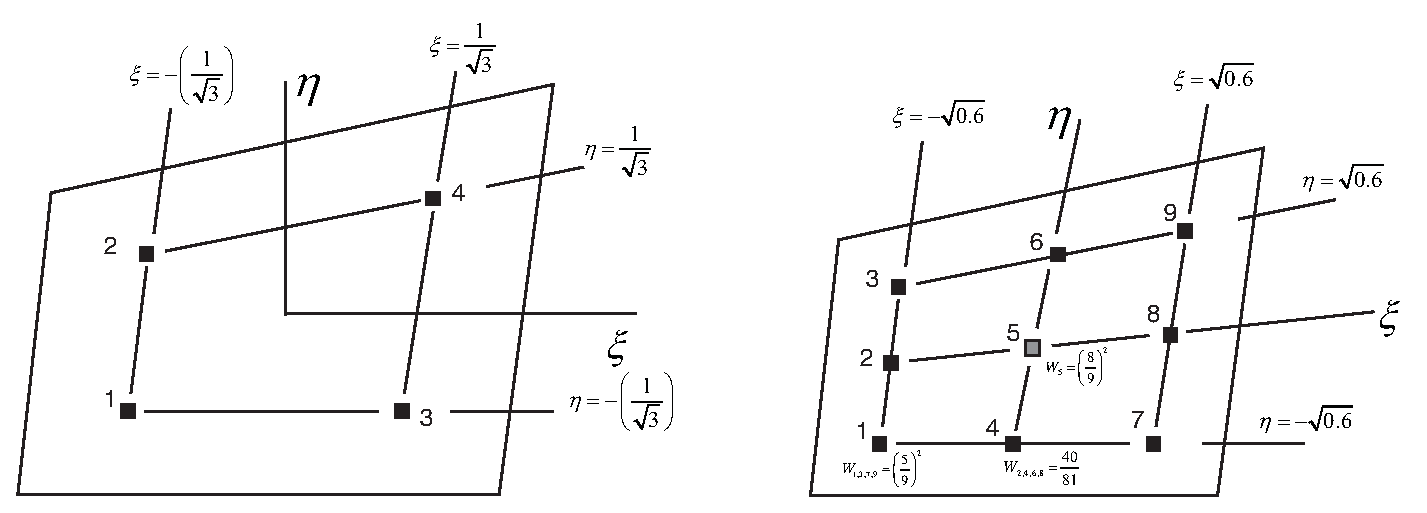
\includegraphics[width=12cm]{fig/gauss_n3.eps}
    \caption{Puntos gauss para ordenes $n=2$ y $n=3$. El peso para $n=2$ es igual en todos los puntos $W_i=1$}
    \label{fig:gauss_n3}
\end{figure}
\subsection{Ejemplo elemento exótico}
\subsubsection*{Matriz de Rigidez}
Imaginemos un elementos Q5 cuadrado de $2\times2$ con espesor $t$  (igual al Q4 con un nodo en su centro). Si fuéramos a obtener las funciones de formas de dicho elemento quedarían iguales para $(x,y)$ y para $(\xi,\eta)$ por las dimensiones usadas. La funcionalidad que uno estaría tentado a seleccionar sería $[1\ x \ y\ x^2 \ y^2 ]$, pero está trae problemas inesperados debido a que tiene varias soluciones en la interpolación. Como nuestra prioridad siempre es mantener la simetría la funcionalidad será $[1\ x\ y\ xy\ x^2y^2 ]$.  Tomando el orden de la figura \ref{fig:elemq5}.
\[
N_i=\left[\begin{array}{ccccc} \frac{x^2\,y^2}{4}+\frac{x\,y}{4}-\frac{x}{4}-\frac{y}{4}, & \frac{x^2\,y^2}{4}-\frac{x\,y}{4}+\frac{x}{4}-\frac{y}{4}, & \frac{x^2\,y^2}{4}+\frac{x\,y}{4}+\frac{x}{4}+\frac{y}{4}, & \frac{x^2\,y^2}{4}-\frac{x\,y}{4}-\frac{x}{4}+\frac{y}{4}, & 1-x^2\,y^2 \end{array}\right]
\]

Llegado a este punto nos interesa obtener la matriz de rigidez. Si queremos lograr \emph{``full integration"} deberíamos usar Gauss orden $n=3$ según $2n-1\geq O\left(\MB^T \ME \MB \right)$. El producto $\MB^T \ME \MB$ da un polinomio de orden 6 ($\MB$ tiene el mismo orden que la derivada de $\MN$). De esta forma nos aseguramos que nuestro resultado va ser exacto para el elemento sin distorsionar.

Para esté ejemplo, no se pide \emph{full integration} entonces no pasa nada si queremos \emph{underintegrate}. Usamos Gauss orden $n=2$. 

\begin{figure}[htb!]
    \centering
    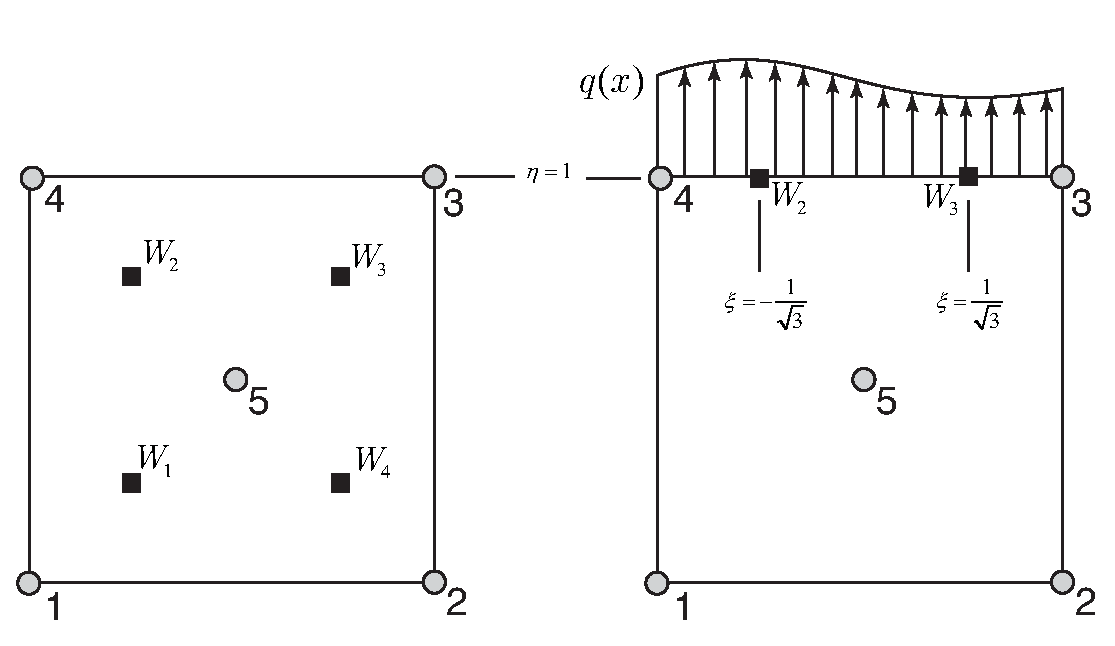
\includegraphics[height=5cm]{fig/exoticElement.eps}
    \caption{Elemento Q5 rectangular.}
    \label{fig:elemq5}
\end{figure}

La rigidez de un elemento está dada por 


\begin{equation}
    \Mk=\int \MB^T \ME \MB \di V=\iint \MB^T \ME \MB t \di x \di y=\int^1_{-1}\int^1_{-1} \MB^T \ME \MB t \ \Djac \  \di\xi  \di\eta
\end{equation}
donde $\MB$ es la matriz deformación-desplazamiento del elemento, $\ME$ es la matriz constitutiva, y $\Djac$ es el determinante de la matriz Jacobiana, el cual se le suele decir simplemente el Jacobiano.

Este ultimo se calcula a partir de la derivada de las funciones de forma $ $

\subsubsection*{Cargas 2-D}
La ecuación que rige como se cargan elementos, siendo $\Cme{r}$ las cargas nodales, $\Cme{F}$ fuerzas volumétricas, $\CPhi$ fuerzas de tracción superficiales, $\Cme{\varepsilonb_0}$ las deformaciones iniciales y $\Cme{\sigmab_0}$ las tensiones iniciales (pg. 228)
\begin{equation} \label{eq:CargasGenerales}
    \Cme{r}=\int \MN^T \Cme{F} \di V +\int \MN^T \CPhi \di S+\int \MB^T \ME \Cme{\varepsilonb_0} \di V- \int \MB \Cme{\sigmab_0} \di V
\end{equation}
\textbf{Carga de linea}. Si el elemento está cargado sobre la linea 4-3 con una distribuida $q(x)$ (en [\si{\newton \per \meter}]) entonces procedemos de la siguiente manera según el segundo término de \refp{eq:CargasGenerales}: 

\begin{align}
    r_{xi}&=\int^1_{-1}N_i (\tau \jac_{11}- \sigma \jac_{12})t\di \xi \\
    r_{yi}&=\int^1_{-1}N_i (\sigma \jac_{11}+\tau \jac_{12})t \di \xi 
\end{align}
    donde $\sigma$ es la solicitación normal a la superficie y $\tau$ es la tangencial. Para la fuerza sobre el nodo 4 se tiene
    
    $$r_{y4}= N_4(\xi_2)t\left[\sigma(\xi_2)\; \jac_{11}+\tau(\xi_2)\; \jac_{12}\right] \cdot W_2 + N_4(\xi_3)t\left[\sigma(\xi_3)\; \jac_{11}+\tau(\xi_3)\; \jac_{12}\right]\cdot W_3 $$

    Si consideramos que solo hay una \emph{carga distribuida de linea} a tracción/compresión como indica la figura \ref{fig:elemq5}, se reduce la ecuación anterior
    
    $$ r_{y4} = N_4(\xi_2)\;\jac_{11}\;q(\xi_2) + N_4(\xi_3)\;\jac_{11}\;q(\xi_3) =N_4\;q \;\jac_{11}\Big|_{\xi_2} + N_4\;q\; \jac_{11}\Big|_{\xi_3} $$
    similarmente $r_{y3} = N_3\;q \;\jac_{11}\big|_{\xi_2} + N_3\;q\; \jac_{11}\big|_{\xi_3} $ donde la matriz Jacobiana también se evalúa para cada punto de Gauss!
    
    \textbf{Carga volumétrica}. 
\subsubsection*{Tensiones}
    \begin{itemize}
        \item Las tensiones en los nodos suele ser de mayor interés que sobre los puntos de gauss (mas comprometidas, permiten estimar error)
    \end{itemize}
    \clearpage
%    \subsection*{Código \Matlab{}}
    %%%%------------------------------------------------------------------CODE
    \subsubsection*{Dofinitions}
    \begin{code}
    \begin{verbatim}

%% Definiciones    (N=Número)
Ndofpornod = 2;                    % grados de libertad por nodo
Nelem = size(elementos,1);         % elementos
Nnod = size(nodos,1);           % nodos
Nnodporelem = size(elementos,2);     % nodos por elemento
doftot = Ndofpornodo*Nnod;         % grados de libertad
DOF=reshape(1:doftot,2,[])';    % Matriz de grados de libertad
Ndims = size(nodos,2);          % dimensiones del problema
\end{verbatim}
\end{code}
\subsubsection*{Form Functions}
\begin{code}
\begin{verbatim}

%% Obtención de funciones de forma
syms x y real 
X = [1 x y x^2 x*y y^2]; %LST
A = [1 0 0 0 0 0
     1 1 0 1 0 0
     1 0 1 0 0 1
     1 .5 0 .25 0 0
     1 .5 .5 .25 .25 .25
     1 0 .5 0 0 .25]; 
N = X/A;
dN = [diff(N,x); diff(N,y)];
sum(N);  % == 1
sum(dN,2); % == 0        
\end{verbatim}
\end{code}

\begin{code}[Q8]
	\begin{verbatim}
	
clear dN N dNaux X dNxx dNyy dNxy Bs% Ns2 Ns3 dNs3 dNs2
syms ksi eta real
X = [1 eta ksi ksi.^2 ksi.*eta eta.^2 (ksi.^2).*eta ksi.*(eta.^2)];%
Cambia de Q4 a Q8
% X = [1 ksi eta ksi.*eta];
% w1 t1 t2
Xdx = diff(X,ksi);
Xdy = diff(X,eta);
uNod = [-1 -1
1 -1
1 1
-1 1
0 -1
1 0
0 1
-1 0];
Nnodporelem = length(uNod);
Ndofpornod = 3; %Placas Mindlin
Ndofporelem = Nnodporelem*Ndofpornod;
A = zeros(Nnodporelem,length(X));
for i=1:Nnodporelem
	ksi=uNod(i,1); eta = uNod(i,2);
	A(i,:) = double(subs(X));
end
syms ksi eta real
shapefuns = X*inv(A);
N = shapefuns;
dNx = diff(shapefuns,ksi);
dNy = diff(shapefuns,eta);
dN = [dNx;dNy];     
	\end{verbatim}
\end{code}

\subsubsection*{Preparación para rutina elementos}
\begin{code}
\begin{verbatim}
    
Cstrain = ...
Cstress = ...
Cterm  =  ...
Kglobal = zeros(doftot);
P = zeros(doftot,1); 

fixity = false(doftot,1);
fixity([m n ... z]) = true;
free = ~fixity;

W=[5/9   8/9   5/9]; %El producto W'*W visualiza en 2D los pesos
wpg=reshape(W'*W,[],1);% gauss n=3
\end{verbatim}
\end{code}

\clearpage
\subsubsection*{Matriz rigidez con rutina elementos (tabla 6.3-2)}
\begin{code}
\begin{verbatim}

%% Matriz de rigidez
Kt = zeros(doftotT);
K=zeros(doftot);
jmin = 1E10;
Areas=zeros(Nelem,1);
for iele = 1:Nelem
    A = 0;
    index=elementos(iele,:);
    Ket = zeros(NdofpornodT*Nnodporelem);
    Ke = zeros(Ndofpornodo*Nnodporelem);
    meindof = reshape(DOF(index,:)',1,[]);
    meindofT=DOFT(index)';%ahora lo hago para carga termica
    nodesEle = nodos(index,:);
    for ipg = 1:npg
        ksi = upg(ipg,1);
        eta = upg(ipg,2);
        N = shapefuns([ksi eta],eleType);
        dN = shapefunsder([ksi eta],eleType);
        jac = dN*nodesEle;
        dNxy = jac\dN;       % dNxy = inv(jac)*dN
        B = zeros(size(C,2),Ndofpornodo*Nnodporelem);
        B(1,1:2:Ndofpornodo*Nnodporelem-1) = dNxy(1,:);
        B(2,2:2:Ndofpornodo*Nnodporelem) = dNxy(2,:);
        B(3,1:2:Ndofpornodo*Nnodporelem-1) = dNxy(2,:);
        B(3,2:2:Ndofpornodo*Nnodporelem) = dNxy(1,:);
        Bt=dNxy;%el B para cargas termicas
        Djac = det(jac);
        
        Ke = Ke + B'*C*B*wpg(ipg)*Djac;
        Ket = Ket + Bt'*Ct*Bt*wpg(ipg)*Djac;
        A = A + wpg(ipg)*Djac;
        if Djac < jmin
            jmin = Djac;
        end
    end
    Areas(iele)=A;
    Kt(meindofT,meindofT) = Kt(meindofT,meindofT) + Ket;
    K(meindof,meindof) = K(meindof,meindof) + Ke;
end
\end{verbatim}
\end{code}
\clearpage
\subsubsection*{Carga de Linea Q4 }

\begin{code}
\begin{verbatim}
    
R = zeros(doftot,1);% Vector de cargas
DOF=reshape(1:doftot,2,[])';
surfnod=[4 3];
wpg=[1 1];
a=-sqrt(3)^-1;
upg=[-a 1;a 1];
npg=2;
sig=-.02;
for e=1:Nelem
    index=elementos(e,:);
    meindof=DOF(index,:);
    elenod=nodos(index,:);
    A=elenod(:,2)==60; % y=60 => Cargo
    if  isempty(find(A,1))
        continue
    end
    for ipg=1:npg
        ksi = upg(ipg,1);
        eta = upg(ipg,2);
        N = shapefuns([ksi eta],eleType);
        dN = shapefunsder([ksi eta],eleType);
        jac = dN*elenod;
        W=wpg(ipg);
        for snod=surfnod
           R(meindof(snod,1))=R(meindof(snod,1))+t*N(snod)*(-jac(1,2))*sig*W;
           R(meindof(snod,2))=R(meindof(snod,2))+t*N(snod)*jac(1,1)*sig*W;
           qcheck=qcheck+t*N(snod)*jac(1,1)*sig*W; %Sería de las dos
        end
    end
end
R=reshape(R,2,[])';
\end{verbatim}
\end{code}
    
\subsubsection{Cálculo de tensiones iterando sobre elementos pg. 230}
\begin{code}
\begin{verbatim}

stress = zeros(Nnodporelem,3,Nelem);

meindof=reshape(DOF(index,:)',[],1);
stress(inode,:,iele) = C*B*D(meindof);
%...

S=2; % para sigma_yy
plotvar=squeeze(stress(:,S,:))';
bandplot(elementos,nodePosition,plotvar,[],'k');
\end{verbatim}
\end{code}

\subsubsection{Triangulos pg. 260  Gauss Triangulos (267)}
\begin{code}
\begin{verbatim}
    
%% Gauss grado 2 tringular
a   = 1/2;
upg = [a  0
       0  a
       a  a];    
npg = size(upg,1);
wpg = [1 1 1]/3;
\end{verbatim}
\end{code}
\subsubsection*{Resolución de problema de Calor con tensiones iniciales}
\begin{code}\label{cod:calorDesconocidos}
\begin{verbatim}

Co=[1,6,5,10,11,12,13,14,15];
X=[2,3,4,7,8,9]; %numel(Co)+numel(X)==doftotT
Kxx=Kt(X,X);Kxc=Kt(X,Co);
Tc=zeros(length(Co),1);
Tc([1,2,5])=100;%los nodos con respecto a Co
Rt=Kxc*Tc;
Tx=Kxx\-Rt;
T=zeros(Nnod,1);
T(X)=Tx;
T(Co)=Tc;
for i=1:Nelem
    temp(i,:)=T(elementos(i,:)); %temp es graficable
end
%% Encuentro FUERZAS GENERADAS POR GRADIENTE CALOR(rutina elementos[RE])
index=elementos(iele,:)
R(index,:) = R(index,:) + ...
reshape(-B'*C*(N*T(index)*[1 1 0]')*alfa*wpg(ipg)*Djac,2,Nnodporelem)';
%% Busco D con estás fuerzas con K\R->Tensiones térmicas (RE sobre NODOS)
\end{verbatim}
\end{code}

\subsubsection*{(cont.) Tensiones y flujo de calor. Rutina Elementos para tensiones sobre nodos}
\begin{code}
\begin{verbatim}

uNod = [-1 -1;1 -1;1  1;-1  1];%Q4
q=zeros(Nnodporelem*Ndofpornodo,1);
stress = zeros(Nnodporelem,3,Nelem);
for iele = 1:Nelem
    index = elementos(iele,:);
    nodesEle = nodos(index,:);
    indexT=index;
    meindof = reshape(DOF(index,:)',1,[]);
    TnodosEle=T(index); %Del perfil temp.
    for inod = 1:Nnodporelem
        ksi,eta = uNod(inod,1),uNod(inod,2);
        dN  = shapefunsder([ksi eta],eleType);
%Obtengo jacobiano, B
        stress(inod,:,iele) = C*(B*D(meindof)-(alfa*TnodosEle(inod)*[1 1 0]'));
        q([2*indexT(inod)-1,2*indexT(inod)])=-k*Bt*T(indexT);
    end
end
qx=q(1:2:end);
qy=q(2:2:end);
quiver(nodos(:,1),nodos(:,2),qx,qy) %Plot Quiver
\end{verbatim}
\end{code}

$$
dN_i=\left(\begin{array}{cccccc} 4\,x+4\,y-3, & 4\,x-1, & 0, & 4-4\,y-8\,x, & 4\,y, & -4\,y\\ 4\,x+4\,y-3, & 0, & 4\,y-1, & -4\,x, & 4\,x, & 4-8\,y-4\,x \end{array}\right)_{LST}
$$
\begin{figure}
    \centering
    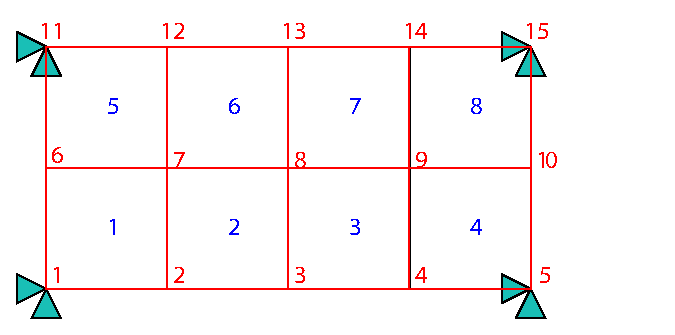
\includegraphics[width=10cm]{fig/problema_calor.eps}
    \caption{Problema depicto en el código \ref{cod:calorDesconocidos}}
    \label{fig:probCalor}
\end{figure}
\section{Parcial 3}

\subsection{Axisimetría}
Resuelvo problema 3-D en el plano. Los resultados son por cada unidad radian. Como sigo teniendo dos grados de libertad tengo las mismas funciones de forma. Cambia mi operador derivada.
\[
\begin{Bmatrix}
    \sigma_\radial \\
    \sigma_\theta \\
    \sigma_z \\
    \tau_{z\radial}
\end{Bmatrix}
= \frac{(1-\nu)E}{(1+\nu)(1-2\nu)}
\begin{bmatrix}
   1 & \eff & \eff & 0 \\
    & 1 & \eff & 0 \\
    & & 1 & 0 \\
    \textrm{sim.}\unspace& & & g 
\end{bmatrix}
\left(
\begin{Bmatrix}
\varepsilon_\radial \\
\varepsilon_\theta \\
\varepsilon_z \\
\gamma_{\radial z}
\end{Bmatrix}
-
\begin{Bmatrix}
\alpha T\\
\alpha T \\
\alpha T \\
0
\end{Bmatrix}
\right)
\]
donde 
\[
f=\frac{\nu}{1-\nu}\qquad \quad \textrm{y}\quad \qquad g=\frac{1-2\nu}{2(1-\nu)}
\]

Una carga puntual $P$ aplicada sobre un elemento axisimétrico no tiene el mismo significado físico que en elementos plane stress/strain. 
\[
P=2\pi rq
\]
donde $q$ es la carga distribuida en [N/m], $r$ es la distancia al eje de revolución y $2 \pi$ es el resultado de integrar la fuerza distribuida sobre $\theta$. 

\[
\Cme{r_e} = \int\int_{-\pi}^{\pi} \MN^T \begin{Bmatrix}
    \rho r \omega ^2 \\
    0
\end{Bmatrix} r \di \theta \di A
\]

\subsection{Subestructuras}
\[
\begin{bmatrix}
    K_{AA} & K_{AB} \\
    K_{BA} & K_{BB}
\end{bmatrix}
\begin{bmatrix}
    D_A \\
    D_B
\end{bmatrix}
= \begin{bmatrix}
    R_A \\
    R_B
\end{bmatrix}
\]

\[ 
D_B = K_{BB}^{-1} (R_B - K_{BA}D_A)
\]
\[
D_A =K_{AA}^{-1}(R_A-K_{AB}D_B)
\]

\subsection{Pitfalls}
\subsubsection*{\Matlab{}}
\begin{itemize}
    \item Antes de aplicar carga distribuida, verificar la orientación del elemento con sus nodos ($\xi,\eta$)
    \item
\end{itemize}
\subsection{Error}
Tipos de error:
\begin{itemize}
    \item Modelado
    \item Bugs
    \item Error de usuario
    \item Error de discretización
    \item Error de redondeo/truncado
    \item Error de manipulación 
    \item Error numérico (combinación de los dos anteriores)
\end{itemize}

Cálculo Tensiones en puntos superconvergencia (Gauss orden 1 para Q4, y Gauss orden 2 aproxima para Q8).

Extrapolo tensiones superconvergentes a los nodos ($\sigma^*$).

Energía de deformación.

Se suele requerir que $\eta\leq 0,05$
\[
\vvert{U}^2 = \sum^m_{i=1}\int_{v_e} \Cme{\varepsilonb}_i^T \ME \Cme{\varepsilonb}_i \di V
\]
\[
\vvert{e}^2=\sum_{i=1}^m \int_{v_e} \left( \Cme{\varepsilonb^*}_i - \Cme{\varepsilonb}_i\right)^T \ME \left( \Cme{\varepsilonb^*}_i - \Cme{\varepsilonb}_i\right) \di V
\]

\[
\vvert{e}^2=\sum_{i=1}^m \int_{v_e} \left( \Cme{\sigmab^*}_i - \Cme{\sigmab}_i\right)^T \ME ^{-1} \left( \Cme{\sigmab^*}_i - \Cme{\sigmab}_i\right) \di V
\]

\[
\eta = \sqrt{\frac{\vvert{e}^2}{\vvert{e}^2+\vvert{U}^2}}
\]




% \subsection*{Código \Matlab{}}
    %%%%------------------------------------------------------------------CODE
    \subsubsection*{Código Axisimétrico para matriz rigidez (por radian)}
    Se va tratar con un método para el almacenado eficiente de las funciones de forma. Esto acorta el tiempo de corrido en un factor mayor a 100 para problemas medianos/grandes. Se puede tambien hacer para los nodos (código )
    \begin{code}
    \begin{verbatim}

%% ALMACENADO EFICIENTE
Ns=cell(npg,1); %Acelerar proceso.
dNs=cell(npg,1);
NLs=cell(npg,1);
for ipg=1:npg
    ksi=upg(ipg,1);eta=upg(ipg,2);
    Ns{ipg}=eval(subs(N));
    dNs{ipg}=eval(subs(dN));
    NLs{ipg}=eval(subs(NL));
end
    \end{verbatim}
    \end{code}
    
    \begin{code}
    \begin{verbatim}
    
kG=zeros(doftot);%Matriz global
for e=1:Nelem
    Ke=zeros(Ndofpornod*Nnodporelem);
    index=elementos(e,:);
    elenod=nodos(index,:);
    A=0;
    for ipg=1:npg
        ksi=upg(ipg,1); eta=upg(ipg,2);

        J=dNs{ipg}*elenod;
        Djac = det(J);
        dNxy=J\dNs{ipg};
        r = Ns{ipg}*elenod(:,1); 
        
        B = zeros(size(Caxi,2),Ndofpornod*Nnodporelem);
        B(1,1:2:Ndofpornod*Nnodporelem-1) = dNxy(1,:);
        B(2,1:2:Ndofpornod*Nnodporelem-1) = Ns{ipg}(1,:)/r;
        B(3,2:2:Ndofpornod*Nnodporelem) = dNxy(2,:);
        B(4,1:2:Ndofpornod*Nnodporelem-1) = dNxy(2,:);
        B(4,2:2:Ndofpornod*Nnodporelem) = dNxy(1,:);%extra fila por ser axisim.

        Ke = Ke + B'*Caxi*B*wpg(ipg)*r*Djac;%Despues aplicar cargas por radian
    end
    meindof=reshape(DOF(index,:)',1,[]);
    kG(meindof,meindof)=kG(meindof,meindof)+Ke;
end
\end{verbatim}
\end{code}

\subsubsection*{Recuperación de tensiones axisimétricas.}
\begin{code}
\begin{verbatim}
 
for e = 1:Nelem
    index = elementos(e,:);
    elenod = nodos(index,:);
    for inod = 1:Nnodporelem
        J = dNs{inod}*elenod;                  

        dNxy = J\dNs{inod};     
        r = Ns{ipg}*elenod(:,1);
        
        B = zeros(size(C,2),Ndofpornod*Nnodporelem);
        B(1,1:2:Ndofpornod*Nnodporelem-1) = dNxy(1,:);
        B(2,1:2:Ndofpornod*Nnodporelem-1) = Ns{inod}(1,:)/r;
        B(3,2:2:Ndofpornod*Nnodporelem) = dNxy(2,:);
        B(4,1:2:Ndofpornod*Nnodporelem-1) = dNxy(2,:);
        B(4,2:2:Ndofpornod*Nnodporelem) = dNxy(1,:);
        
        meindof = reshape(DOF(index,:)',1,[]);
        
        deformation = B*D(meindof);
        if r==0
            deformation(2)=deformation(1);
        end
        deformation;
        strain(e,inod,:) = deformation;
        S(e,inod,:) = C*deformation; % Stress
    end
end
\end{verbatim}
\end{code}
\subsubsection*{Carga centrifugas (por radian)}
\begin{code}
\begin{verbatim}

R = zeros(doftot,1);
for e = 1:Nelem
    index=elementos(e,:);
    Re = zeros(Ndofpornod*Nnodporelem,1);
    elenod = nodos(elementos(e,:),:);
    for ipg = 1:npg
        ksi=upg(ipg,1); eta=upg(ipg,2);
        J = dNs{ipg}*elenod;
        r = Ns{ipg}*elenod(:,1);
        
        Re = Re + (NLs{ipg}'*[1; 0])*det(J)*wpg(ipg)*r^2*rho*omega^2;
    end
    meindof=reshape(DOF(index,:)',1,[]);
    R(meindof) = R(meindof) + Re;
end
\end{verbatim}
\end{code}

\subsubsection*{Condicionamiento}
\begin{code}
\begin{verbatim}

CK = max(eigvals)/min(eigvals)
N=size(K,2);
S=zeros(N);
for i=1:N
    S(i,i)=sqrt(K(i,i))^(-1);
end
Ks=S*K*S;
scaledeigval=eig(Ks);
CKscaled=max(scaledeigval)/min(scaledeigval)
digitos_perdidos = floor(log10(CKscaled))
\end{verbatim}
\end{code}

\subsubsection*{Desplazamientos impuestos sin \emph{skew}}
\begin{code}
\begin{verbatim}

% Solve sin cargas por despl. impuestos
Dr = Kr\Rr;
%% Buscamos imponer desplazaments iniciales
dx=-sqrt(2);
dy=dx;
Dc=zeros(doftot,1);
CONOC=Fixed;
CONOC([9 10 11]*Ndofpornod)=true;
CONOC([9 10 11]*Ndofpornod-1)=true;
DECONOC=~CONOC;
Dc([9 10 11]*Ndofpornod)=dy;
Dc([9 10 11]*Ndofpornod-1)=dx;

Dx = K(DECONOC,DECONOC)\(R(DECONOC)-K(DECONOC,CONOC)*Dc(CONOC));
Rx = K(CONOC,CONOC)*Dc(CONOC)+K(CONOC,DECONOC)*Dx;
R(CONOC)=Rx;
Dc(DECONOC)=Dx;
D=Dc;
%Voy a recuperacion de tensiones
\end{verbatim}
\end{code}
\subsubsection*{Despl. impuestos con \emph{skew}}
\begin{code}
\begin{verbatim}

%Solve sin despl. impuestos
Dr = Kr\Rr;
%% SKEW SYSTEM Desp. imp.
T = eye(doftot);angulo =45;
for i = [9 10 11]
    nodedof = [i*2-1 i*2];
    T(nodedof,nodedof)=[cosd(angulo) sind(angulo); ...
    -sind(angulo) cosd(angulo)];
end
Dc = nan(doftot,1); Dc([1 2 3 9 10 11]*Ndofpornod)=0;
Dc([9 10 11]*Ndofpornod-1)=-2;
XX=isnan(Dc);CC=~XX; %DesConocidas y Conocidas
%Resuelvo
Kskew = T*K*T'; Rskew = T*R;
Dx = Kskew(XX,XX)^(-1)*(Rskew(XX)-Kskew(XX,CC)*Dc(CC));
Rskew(CC) = Kskew(CC,CC)*Dc(CC)+Kskew(CC,XX)*Dx;

%Ahora son TODOS conocidos jeje
Dc(XX)=Dx; % AhDesde ahora isnan(Dc)=0!

D=T'*Dc;
Desp = reshape(D',Ndofpornod,Nnod)';
% Directo a Recuperacio de tensiones en nodos.
\end{verbatim}
\end{code}

\subsubsection*{Error Q8}

\begin{code}
\begin{verbatim}

%% tensiones en los puntos de superconvergencia
stressSuper = zeros(nel,4,3);
uNod = [-1 -1
1 -1
1 1
-1 1]/sqrt(3);
for iele = 1:nel
nodesEle = nodes(elements(iele,:),:);
for inode = 1:4
% Punto de Gauss
ksi = uNod(inode,1);
eta = uNod(inode,2);
% Derivadas de las funciones de forma respecto de ksi, eta
dN = shapefunsder([ksi eta],'Q8');
% Derivadas de x,y, respecto de ksi, eta
jac = dN*nodesEle;
% Derivadas de las funciones de forma respecto de x,y.
dNxy = jac\dN; % dNxy = inv(jac)*dN

B = zeros(size(C,2),nDofNod*nNodEle);
B(1,1:2:15) = dNxy(1,:);
B(2,2:2:16) = dNxy(2,:);
B(3,1:2:15) = dNxy(2,:);
B(3,2:2:16) = dNxy(1,:);
eleDofs = nodeDofs(elements(iele,:),:);
eleDofs = reshape(eleDofs',[],1);
stressSuper(iele,inode,:) = C*B*D(eleDofs);
end
end
% Extrapolo a los Nodos
a = sqrt(3);
rsExt = a*[-1 -1
1 -1
1 1
-1 1
0 -1
1 0
0 1
-1 0];
stressExtra = zeros(nel,nNodEle,3);
for iele = 1:nel
    for inode = 1:nNodEle
        r = rsExt(inode,1);
        s = rsExt(inode,2);
        N = shapefuns([r s],'Q4');
        stressExtra(iele,inode,:) = N * squeeze(stressSuper(iele,:,:));
    end
end
%% Gauss
[wpg, upg, npg] = gauss([3 3]);
%% calculo de eta_el, e2, U2
invC = C\eye(3);
eta_el = zeros(nel,1);
e2_el = zeros(nel,1);
U2_el = zeros(nel,1);
for iele = 1:nel
    nodesEle = nodes(elements(iele,:),:);
    for inode = 1:nNodEle
        for ipg = 1:npg
            % Punto de Gauss
            ksi = upg(ipg,1);
            eta = upg(ipg,2);
            % Derivadas de las funciones de forma respecto de ksi, eta
            dN = shapefunsder([ksi eta],'Q8');
            % Derivadas de x,y, respecto de ksi, eta
            jac = dN*nodesEle;
            % Derivadas de las funciones de forma respecto de x,y.

            dNxy = jac\dN; % dNxy = inv(jac)*dN
            % funciones de forma
            N = shapefuns([ksi eta],'Q8');
            eleStress = squeeze(stress(iele,inode,:)); %
            tensiones "directas"
            starStress = squeeze(stressExtra(iele,inode,:)); %Str.mejoradas
            e2_el(iele) = e2_el(iele) + (starStress - eleStress)' * ...
            invC * (starStress - eleStress) * wpg(ipg) *det(jac);

            U2_el(iele) = U2_el(iele) + eleStress' * invC * eleStress * ...
            wpg(ipg) * det(jac);
        end
    end
    eta_el(iele) = sqrt( e2_el(iele) / (e2_el(iele) + U2_el(iele)) );
end
etaG = sqrt( sum(e2_el) / (sum(e2_el) + sum(U2_el)) )
%% Configuracion deformada
D = (reshape(D,nDofNod,[]))';
nodePosition = nodes + D(:,1:2);
%Graficacion
limites = [min(min(stressExtra(:,:,2))),max(max(stressExtra(:,:,2)))];
figure(1)
bandplot(elements,nodePosition,stress(:,:,2),limites,'k');
\end{verbatim}
\end{code}
\subsubsection*{\Adina}
\begin{figure}[htb!]
    \centering
    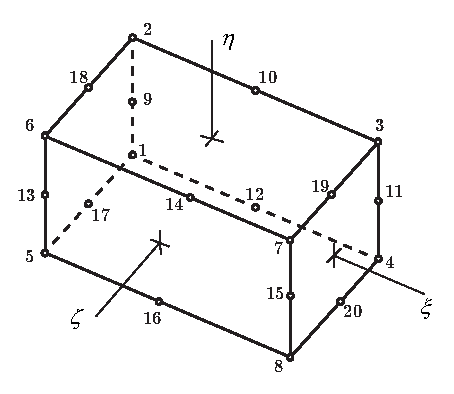
\includegraphics[width=.6\textwidth]{fig/H20numbering.eps}
    \caption{Numeración de nodos H20 en \Adina (Ejes sugeridos)}
    \label{fig:H20numbering}
\end{figure}

\section{Finitos II}
Modal:
\[
\Cme{Z} = \frac{\Cme{R\modal }}{{\COmega}^2 \sqrt{(1-\chi^2)^2 + (2 \dampfact \chi)^2}}
\]
donde $\chi = \frac{\omega_{\mathrm{exc}}}{\COmega}$ y $\dampfact$ se elige por el usuario.
\\
\\
Proporcional:

\[
\Cme{D} = \frac{\Cme{R }}{{\COmega}^2 \sqrt{(1-\chi^2)^2 + (2 \dampfact \chi)^2}}
\]
donde $\chi = \frac{\omega_{\mathrm{exc}}}{\COmega}$ y 
$\dampfact = \tfrac{1}{2} \left(\frac{\alpha}{\omega_{\mathrm{exc}}} +\beta \omega_{\mathrm{exc}} \right) $

Si se quiere estudiar un rango de frecuencias de excitación tal que $\omega_{\mathrm{exc}}\in [\omega_1, \omega_2]$ y eligiendo dos valores de damping para ambas frecuencias $\dampfact_1$ y $\dampfact_2$ se tiene:
\begin{align*}
	\alpha &= 2\omega_1 \omega_2 (\dampfact_1 \omega_2 -\dampfact_2 \omega_1)/(\omega_2^2 - \omega_1^2) \\ \beta &= 2(\dampfact_2\omega_2 -\dampfact_1 \omega_1)/(\omega_2^2 - \omega_1^2)
\end{align*}


\subsection{Sine Sweep}
A medida que la frecuencia de excitación aumenta la \textit{amplitud del sistema disminuye}\footnote{Excepto en cercanías de una frecuencia natural}. Es interesante pensar que si aumentara no tendría sentido buscar las frecuencias naturales porque estas son caracterizadas por un máximo de amplitud. Las curvas del barrido de frecuencia son decrecientes en lejanía de una frecuencia natural porque para una fuerza cíclica $F(t)=F_0\sin \omega t$ el tiempo que actúa en una dirección es inversamente proporcional a la frecuencia. Por ende la estructura no tiene tiempo para moverse lejos antes de que se invierta la dirección de la fuerza.
 \clearpage
 \subsection*{Código \Matlab{} Finitos II}
    %%%%------------------------------------------------------------------CODE
    \subsubsection*{Código de Placas}
    Se va tratar con un método para el almacenado eficiente de las funciones de forma usando structures de \Matlab{}. Esto acorta el tiempo de corrido en un factor mayor a 100 para problemas medianos/grandes. Código en anexo.

    \begin{code}[Funciones de Forma Mindlin Q4]
    \begin{verbatim}

clear dN N dNaux X dNxx dNyy dNxy 
syms ksi eta real
X = [1 ksi eta ksi.*eta];
Xdx = diff(X,ksi);
Xdy = diff(X,eta);
uNod = [-1 -1;1 -1;1 1;-1 1];
Nnodporelem = length(uNod);
Ndofpornod = 3; %Placas Mindlin
Ndofporelem = Nnodporelem*Ndofpornod;
A = zeros(Nnodporelem,length(X));
for i=1:Nnodporelem
  ksi=uNod(i,1); eta = uNod(i,2);
  A(i,:) = double(subs(X));
end

syms ksi eta real
shapefuns = X*inv(A);
N = shapefuns;
dNx = diff(shapefuns,ksi);
dNy = diff(shapefuns,eta);
B =  sym('noImporta',[5,Ndofporelem]);
for i = 1:Nnodporelem
  B(:,(i*3-2):(i*3)) = [0 dNx(i) 0;0 0 dNy(i);0 dNy(i) dNx(i);
	-dNx(i) N(i) 0;-dNy(i) 0 N(i)];
end
dN = [dNx;dNy];
    \end{verbatim}
    \end{code}

\begin{code}[Dofinitions y elemDof]
	\begin{verbatim}

[Nelem, Nnodporelem]= size(elementos);  
[Nnod, Ndim] = size(nodos); % Numero de nodos, Numero de dimensiones del problema (es 2-D)

Ndofpornod = 3; %Para placa Kirchoff
dof = Nnod*Ndofpornod;
DOF = (1:dof)'; %vector columna

n2d = @(nodo) [nodo*3-2, nodo*3-1, nodo*3]; % Función Node a DOF. Obtiene indices de dof de un nodo. Si hay mas/menos de 3 dof por nodo entonces cambia
elemDof = zeros(Nelem,Ndofpornod*Nnodporelem);
for e = 1:Nelem
for n = 1:Nnodporelem
  elemDof(e,n2d(n)) = n2d(elementos(e,n));
end
end
	\end{verbatim}
\end{code}

\begin{code}[Constitutiva]
	\begin{verbatim}
	
F = E*t^3/(12*(1 - NU^2)); %Rigidez ante la flexion
G = E/(2+2*NU); % Rigidez a la torsion
Cb = [F NU*F 0;
NU*F F 0 
0 0 (1-NU)*F/2];
Cs = 5/6*[G*t 0;0 G*t];
C = blkdiag(Cb,Cs);
	\end{verbatim}
\end{code}

\begin{code}[Acople matriz rigidez]
	\begin{verbatim}
	
Kg = sparse(dof,dof);
for e = 1:Nelem
  Kb = zeros(Ndofporelem);
  dofIndex = elemDof(e,:);
  storeTo = elemDof(e,:);
  nodesEle = nodos(elementos(e,:),:);
  Bb = zeros(3,Ndofporelem);
  Bs = zeros(2,Ndofporelem);
  for ipg = 1:npg2
    ksi = upg2(ipg,1); eta = upg2(ipg,2);
    jac = dNs2{ipg}*nodesEle;
    dNxy = jac\dNs2{ipg};   % dNxy = inv(jac)*dN
    for i = 1:Nnodporelem 
     Bb(:,(i*3-2):(i*3)) = [0 dNxy(1,i) 0;0 0 dNxy(2,i);0 dNxy(2,i) dNxy(1,i)];
    end
    Kb = Kb + Bb'*Cb*Bb*wpg2(ipg)*det(jac);
  end
  jac = dNs1*nodesEle;
  dNxy = jac\dNs1;   % dNxy = inv(jac)*dN
  for i = 1:Nnodporelem 
    Bs(:,(i*3-2):(i*3)) = [-dNxy(1,i) Ns1(i) 0;-dNxy(2,i) 0 Ns1(i)];
  end
  Ks = Bs'*Cs*Bs*wpg1*det(jac);

  Kg(storeTo,storeTo) = Kg(storeTo,storeTo) + Kb+ Ks;
end
	\end{verbatim}
\end{code}

\begin{code}[Cargas]
	\begin{verbatim}
	
p0 = -0.05e6; %MPa
R = zeros(dof,1);
for e = 1:Nelem
   storeTo = elemDof(e,1:3:end);
   nodesEle = nodos(elementos(e,:),:);
   for ipg = 1:npg2
     jac = dNs2{ipg}*nodesEle;
     Q = Ns2{ipg}'*p0*wpg2(ipg)*det(jac);
     R(storeTo)=R(storeTo)+Q;
  end
end
	\end{verbatim}
\end{code}

\begin{code}[Recuperación de tensiones]
	\begin{verbatim}
	
Sb = zeros(Nnodporelem,3,Nelem);
Ss = zeros(Nnodporelem,2,Nelem);
% FuncFormas en nodos
Nsn = cell(Nnodporelem,1);
dNsn = cell(Nnodporelem,1);
for inod = 1:Nnodporelem
  ksi = uNod(inod,1); eta = uNod(inod,2);
  dNsn{inod} = double(subs(dN));
  Nsn{inod} = double(subs(N));
end

for e = 1:Nelem
  storeTo = elemDof(e,:);
  nodesEle = nodos(elementos(e,:),:);
  Bb = zeros(3,Ndofporelem);
  Bs = zeros(2,Ndofporelem);
  for  inod = 1:Nnodporelem
    ksi = uNod(inod,1); eta = uNod(inod,2);
    Nder=dNsn{inod};
    jac = Nder*nodesEle;
    dNxy = jac\Nder;  % dNxy = inv(jac)*dN     
    for i = 1:Nnodporelem % Armo matriz B de bending
        Bb(:,(i*3-2):(i*3)) = [0 dNxy(1,i) 0
        0 0 dNxy(2,i)
        0 dNxy(2,i) dNxy(1,i)];
    end
    for i = 1:Nnodporelem 
      Bs(:,(i*3-2):(i*3)) = [-dNxy(1,i) Nsn{inod}(i) 0
     -dNxy(2,i) 0 Nsn{inod}(i)]; % Ver cook 15.3-3
    end
    Sb(inod,:,e) = Cb*(Bb*D(storeTo));
    Ss(inod,:,e) = Cs*(Bs*D(storeTo));
  end
end
	\end{verbatim}
\end{code}

\begin{code}[Plot Von Mises y desplazamientos]
	\begin{verbatim}
	
Svm1 = (((Sb(:,1,:)-Sb(:,2,:)).^2+(Sb(:,3,:).^2 + ...
   Ss(:,1,:).^2+Ss(:,2,:).^2) )./2).^(.5);
bandplot(elementos,nodos,squeeze(Svm1)',[],'k')

Dz = zeros(divisionesx,divisionesy); % Matriz superficie
xv =[];
yv = [];
for n=1:Nnod
   xv = [xv nodos(n,1)];yv = [yv nodos(n,2)];
   Dz(n) = D(n*3-2);
end
Dz=reshape(Dz,[],1)';
scatter3(xv,yv,Dz)
	\end{verbatim}
\end{code}

\subsubsection{Vibraciones}
La rutina para acoplar a la matriz de rigidez y la matriz es la misma.
\begin{code}[Matriz de masa  viga 2 dof]
	\begin{verbatim}
	
Me= m/420 * [156    22*Le     54      -13*Le
   22*Le    4*Le^2    13*Le    -3*Le^2
   54      13*Le     156     -22*Le
  -13*Le   -3*Le^2   -22*Le   4*Le^2];
	\end{verbatim}
\end{code}


\begin{code}[El problema de autovalores]
	\begin{verbatim}
	
A = Mg(isFree,isFree)\Kg(isFree,isFree);
[Vr, eigVal]=eig(A);
V=zeros(dof);
V(isFree,isFree)=Vr;
dofred = size(Vr,2);
	\end{verbatim}
\end{code}


\begin{code}[5 formas de obtener $\COmega $]
	\begin{verbatim}
	
Phi = zeros(dofred,dofred);
omega = zeros(dofred,1);
omegaray = zeros(dofred,1);
ray = zeros(dofred,1);
for i = 1:dofred
   Dbi=Db(:,i);
   Phi(:,i) = Dbi/sqrt(Dbi'*Mr*Dbi);
   Phii = Phi(:,i); 
   omegaray(i) = sqrt((Dbi' * Kg(isFree,isFree) *Dbi)/aux);% Cook (11.4-13)
   ray(i)= sqrt((Phii' * Kg(isFree,isFree) *Phii)/(Phii' *...
        Mg(isFree,isFree) *Phii)); %Cook (11.7-1)b
   omega(i) = sqrt(Phii'* Kg(isFree,isFree)*Phii); % Idem
end
ESP  = Phi' * Kg(isFree,isFree) *Phi;
omegaespectral = sqrt(diag(ESP));
omegaeig = sqrt(diag(eigVal)); %y una quinta para que tengas
	\end{verbatim}
\end{code}

\begin{code}[Rutina barrido de frecuencia]
	\begin{verbatim}
	
input_ksi = 0.05:0.05:0.3;
Nmodos = 3;
input_omega = 1:1:10000;
for k = 1:Nksi
   ksi = input_ksi(k);
   for f = 1:Nfrec
      Z=zeros(dofred,1);
      for i=1:dofred
         chi = input_omega(f)/omega(i);
         z(i) = (Rmodalenfrecuencia(i,f)/omega(i)^2)/ ...
              sqrt((1-chi^2)^2+(2*input_ksi(k)*chi)^2);
      end
      Amp(f,k) = abs(sum(z));
   end
   semilogy(input_omega/(2*pi),Amp(:,k))% HZ
   hold on
end
	\end{verbatim}
\end{code}





 \clearpage
 \subsection*{Código \Matlab{} Anexo}
    %%%%------------------------------------------------------------------CODE
    \subsubsection*{Algoritmo rápido para funciones de formas simbólicas}

\begin{code}[aplicación a Gauss $2\times 2$]
	\begin{verbatim} 

k   = 1/sqrt(3);
upg2 = [ -k  -k
          k  -k
          k   k
         -k   k ];
npg2 = size(upg2,1);
wpg2 = ones(npg2,1);

Ns2 = cell(npg2,1);
dNs2 = cell(npg2,1);
for ipg = 1:npg2
   ksi = upg2(ipg,1); eta = upg2(ipg,2);
   dNs2{ipg} = double(subs(dN)); 
   Ns2{ipg} = double(subs(N));
end
	\end{verbatim}
\end{code}

\subsubsection{Matriz de transformación para elementos 1D}
\begin{code}[Barra. $\phi$ en grados]
	\begin{verbatim}
	
T=[cosd(phi) 0;
 sind(phi) 0;
 0 cosd(phi);
 0 sin(phi)];
	\end{verbatim}
\end{code}

\begin{code}[Viga 3 dof por nodo. $\phi$ en grados]
	\begin{verbatim}

T=[cosd(phi) sind(phi) 0 0 0 0;
  -sind(phi) cosd(phi) 0 0 0 0;
   0 0 1 0 0 0;
   0 0 0 cosd(phi) sind(phi) 0;
   0 0 0 -sind(phi) cosd(phi) 0;
   0 0 0 0 0 1];
	\end{verbatim}
\end{code}



\end{document} 




% \begin{comment}
%     \section{Dudas}
%     \begin{enumerate}
%         \item Pg. 223 Cook: $\Mk$ de un solido 8 nodos se integra con $n=2$, pero $\MB$ se integra con $n=3$. Pero se necesita $\MB$ para obtener $\Mk$.
%         \item Si quiero verificar calidad de un elemento, me basta con pararme arriba cada punto Gauss y verificar que $\Djac$ no sea igual a cero y que no cambie de signo?
%         \item Tengo un problema plain strain pero tengo $q(x)$ en [N/m]. No lo integro con $t$! No? Inversamente, para el mismo problema, si tengo solo presiones o fzas volumetricas puedo olvidarme que existe $t$ y no usarla para el calculo de la matriz rigidez (y presiones/fzas vol). Se le dice singularidad a un punto donde $\Djac$ es cero?
%         \item Si quiero tensiones en puntos Gauss, cambia la dimension de $\MB$ cuando itero sobre los puntos? Cook dice que $\MB$ is calculated from (lower order) displacement field. wtf?
%         \item \textbf{Follow-up} Cuando itero sobre los mismos Puntos de Gauss para obtener tensiones, cambian mis $\MN$? Sé que puedo usar los puntos de Gauss para extrapolar tensiones en los nodos, pero hablo antes de eso
%         \item Para un elemento me conviene siempre ser perfectamente simétrico en la elección del orden del polinomio? Hay alguna vez que voy a tomar $[1\ms x\ms y\ms xy\ms x^2]$ antes de tomar algo por el estilo de  $[1\ms x\ms y\ms y^2\ms x^2]$
%     \end{enumerate}
%     \end{comment}